\tikzset{every picture/.style={line width=0.75pt}} %set default line width to 0.75pt        

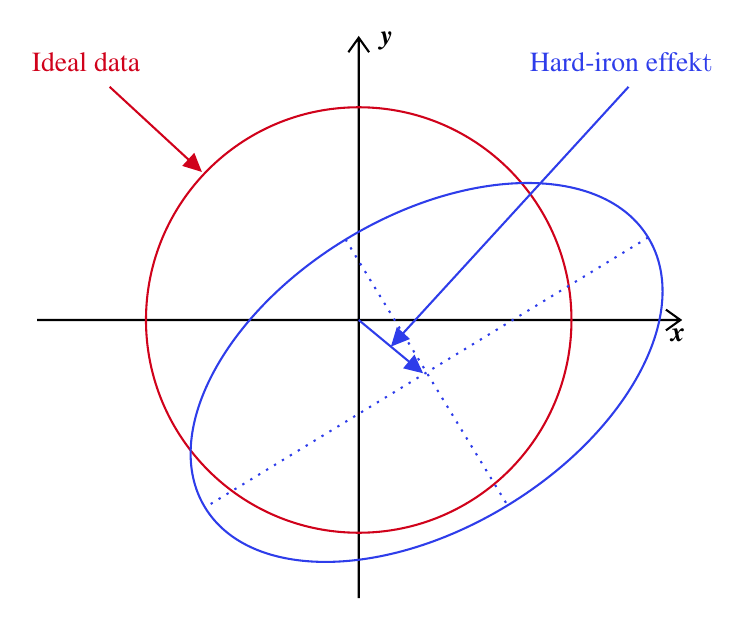
\begin{tikzpicture}[x=0.75pt,y=0.75pt,yscale=-1,xscale=1]
%uncomment if require: \path (0,483); %set diagram left start at 0, and has height of 483

%Shape: Axis 2D [id:dp8169826277465562] 
\draw  (46,256.01) -- (356,256.01)(201,120) -- (201,390) (349,251.01) -- (356,256.01) -- (349,261.01) (196,127) -- (201,120) -- (206,127)  ;
%Shape: Circle [id:dp428612154440116] 
\draw  [color={rgb, 255:red, 208; green, 2; blue, 27 }  ,draw opacity=1 ] (98.5,256.01) .. controls (98.5,199.4) and (144.39,153.51) .. (201,153.51) .. controls (257.61,153.51) and (303.5,199.4) .. (303.5,256.01) .. controls (303.5,312.62) and (257.61,358.51) .. (201,358.51) .. controls (144.39,358.51) and (98.5,312.62) .. (98.5,256.01) -- cycle ;
%Shape: Ellipse [id:dp6713217605276951] 
\draw  [color={rgb, 255:red, 46; green, 61; blue, 234 }  ,draw opacity=1 ] (194.67,217.23) .. controls (253.63,181.31) and (318.89,180.87) .. (340.44,216.25) .. controls (361.99,251.62) and (331.67,309.41) .. (272.71,345.33) .. controls (213.75,381.25) and (148.49,381.69) .. (126.94,346.31) .. controls (105.39,310.94) and (135.71,253.14) .. (194.67,217.23) -- cycle ;
%Straight Lines [id:da9026440537744929] 
\draw [color={rgb, 255:red, 208; green, 2; blue, 27 }  ,draw opacity=1 ]   (81,143.67) -- (123.22,182.64) ;
\draw [shift={(125.43,184.67)}, rotate = 222.7] [fill={rgb, 255:red, 208; green, 2; blue, 27 }  ,fill opacity=1 ][line width=0.08]  [draw opacity=0] (8.93,-4.29) -- (0,0) -- (8.93,4.29) -- cycle    ;
%Straight Lines [id:da006612456158881175] 
\draw [color={rgb, 255:red, 46; green, 61; blue, 234 }  ,draw opacity=1 ]   (331,143.67) -- (218.52,266.62) ;
\draw [shift={(216.5,268.84)}, rotate = 312.45] [fill={rgb, 255:red, 46; green, 61; blue, 234 }  ,fill opacity=1 ][line width=0.08]  [draw opacity=0] (8.93,-4.29) -- (0,0) -- (8.93,4.29) -- cycle    ;
%Straight Lines [id:da17622448909707056] 
\draw [color={rgb, 255:red, 46; green, 61; blue, 234 }  ,draw opacity=1 ] [dash pattern={on 0.84pt off 2.51pt}]  (194.67,217.23) -- (272.71,345.33) ;
%Straight Lines [id:da5489547597587872] 
\draw [color={rgb, 255:red, 46; green, 61; blue, 234 }  ,draw opacity=1 ] [dash pattern={on 0.84pt off 2.51pt}]  (340.44,216.25) -- (126.94,346.31) ;
%Straight Lines [id:da04446912057214236] 
\draw [color={rgb, 255:red, 46; green, 61; blue, 234 }  ,draw opacity=1 ]   (201,256.01) -- (229.69,279.75) ;
\draw [shift={(232,281.67)}, rotate = 219.62] [fill={rgb, 255:red, 46; green, 61; blue, 234 }  ,fill opacity=1 ][line width=0.08]  [draw opacity=0] (8.93,-4.29) -- (0,0) -- (8.93,4.29) -- cycle    ;

% Text Node
\draw (42,125.67) node [anchor=north west][inner sep=0.75pt]  [color={rgb, 255:red, 208; green, 2; blue, 27 }  ,opacity=1 ] [align=left] {{\fontfamily{ptm}\selectfont Ideal data}};
% Text Node
\draw (282,125.67) node [anchor=north west][inner sep=0.75pt]  [color={rgb, 255:red, 46; green, 61; blue, 234 }  ,opacity=1 ] [align=left] {{\fontfamily{ptm}\selectfont Hard-iron effek}t};
% Text Node
\draw (210,115.67) node [anchor=north west][inner sep=0.75pt]   [align=left] {\textit{{\fontfamily{ptm}\selectfont \textbf{y}}}};
% Text Node
\draw (350,258.67) node [anchor=north west][inner sep=0.75pt]   [align=left] {\textit{{\fontfamily{ptm}\selectfont \textbf{x}}}};


\end{tikzpicture}